\documentclass[5pt]{article}
\usepackage{multicol,multirow}
\usepackage{graphicx} % Required for inserting images
\usepackage[margin=0.75cm]{geometry}
\usepackage{xcolor}
\usepackage{amsmath,esint}
\usepackage{mathtools}
\usepackage{relsize}


\usepackage{empheq}
\usepackage{amsfonts}

\usepackage{tkz-euclide}
\usepackage{tikz}

\definecolor{LightGray}{gray}{0.9}

\usepackage{minted}

\DeclarePairedDelimiter\abs{\lvert}{\rvert}%
\DeclarePairedDelimiter\norm{\lVert}{\rVert}%

\makeatletter
\let\oldabs\abs
\def\abs{\@ifstar{\oldabs}{\oldabs*}}

\newcommand{\tr}[3]{
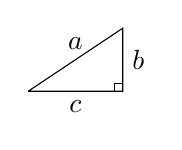
\begin{tikzpicture}[scale=0.40]
    \coordinate [] (A) at (-1.5cm,-1.cm);
    \coordinate [] (C) at (1.5cm,-1.0cm);
    \coordinate [] (B) at (1.5cm,1.0cm);
    \draw (A) -- node[above] {$a$} (B) -- node[right] {$b$} (C) -- node[below] {$c$} (A);
    \draw (1.25cm,-1.0cm) rectangle (1.5cm,-0.75cm);
\end{tikzpicture}
}


\begin{document}


\begin{center}
     \Large{\textbf{Calculus 2 For Engineers}}\\
     \small{Class: APPM 1360}\hfill\small{\textcopyright Maximilien Notz \the\year{}}
     \noindent\rule{20.2cm}{0.4pt}
\end{center}


\begin{multicols}{2}
\setcounter{secnumdepth}{0}


\section{Charges and Fields}
\begin{tabular}{ll}
    Coulomb's Law & $F=k\frac{q_1q_2}{r^2}$ \\
    Definition of electric & $\vec{E}=\frac{\vec{F}_{on q}}{q}$\\
    E-field \footnotesize{(point charge)} & $\vec{E}=k\frac{Q}{r^2}\hat{r}$\\
    E-field \footnotesize{(many charges)} & $\vec{E}_{tot}=\sum\vec{E}=\vec{E}_1+\vec{E}_2+\vec{E}_3+...$\\ 
    E-field \footnotesize{(integral)} & $\vec{E}_{tot}=\int d\vec{E}, d\vec{E}=k\frac{dQ}{r^2}$\\
    Densitys & $dQ=\lambda\;dx=\sigma\;dA=\rho\;dV$
\end{tabular}

\section{Gauss's Law}
\begin{tabular}{ll}
Electric flux & $\Phi=\vec{E}\cdot\vec{A}=\int\vec{E}\cdot d\vec{a}$\\
Gauss Law & $\oiint\vec{E}\cdot d\vec{a}$
\end{tabular}
\section{Electro-Dynamic}
\begin{tabular}{ll}
Voltage          & $v=\frac{\Delta U}{q}$\\
                 & $\Delta U = W_{ext}=- W_{field}$\\
                 & $\Delta U = q\Delta V$\\
                 & $\Delta V=-\vec{E}\cdot\Delta\vec{r}$\\
                 & $W_{ext}=\Delta U =q\Delta V$\\
electric current & $I=\frac{dq}{dt}$\\
Current Density  & $J=\frac{I}{A}=n_eev_{drift}$\\
Ohm's law        & $J=\sigma E$
\end{tabular}

\section{Ciruit}
\begin{tabular}{ll}
Capacitance      & $C=\frac{Q}{V}=\frac{\epsilon_0A}{d}$\\
                 & $U=\frac{1}{2}QV$\\
Electric Current & $I=\frac{dQ}{dt}$\\
Circuits         & $V=IR$\\
                 & $R=\frac{\rho L}{A}$\\
                 & $J=nqV_{drift}=\frac{I}{A}$\\
                 & $P=IV=I^2R=\frac{V^2}{R}$\\
\end{tabular}


\section{Magnetism}
\begin{tabular}{ll}
Definition of \textbf{B} & $F_{on\:q}=q\vec{v}\times\vec{B}$\\
Bio-Savart Law & $d\vec{B}=\frac{\mu_0I}{4\pi}\frac{d\vec{l}\times\hat{r}}{r^2}$\\
Force by a wire & $\vec{F}=I\vec{L}\times\vec{B}$\\
ma
Total force & $\vec{F}_{tot}=\vec{F}_{B} + \vec{F}_{E}$\\
Ampere's Law & $\oint\vec{B}\cdot d\vec{a}=0$\\
Ampere's Law & $\oint\vec{B}\cdot d\vec{l}=\mu_0I_{enclosed}$\\
Faraday's Law & $\mathcal{E}=\oint \frac{\vec{f}_{on\:q}}{q}\cdot d\vec{l}=\oint \vec{E}\cdot d\vec{l}$\\
              & $\mathcal{E}_{N\;loop}=-N\frac{d\Phi_B}{dt}$\\
              

\end{tabular}



\end{multicols}
\end{document}